\documentclass[12pt,a4paper]{article}

\usepackage{inputenc}
\usepackage[english]{babel}
\usepackage[T1]{fontenc}
\usepackage{amsmath}
\usepackage{amsfonts}
\usepackage{amssymb}
\usepackage{graphicx}
\usepackage{epstopdf}
\usepackage{url}
\usepackage{cite}
\usepackage{color}
\usepackage{ifthen}
\usepackage[top=1cm,bottom=0.5cm,right=1cm,left=1cm]{geometry}
\usepackage{algorithm}
\usepackage{algpseudocode}
\usepackage{algorithmicx}
\usepackage{tikz}


%\floatname{algorithm}{Procedure}
\renewcommand{\algorithmicrequire}{\textbf{Input:}}
\renewcommand{\algorithmicensure}{\textbf{Output:}}

%N�cessite les packages "color" et "ifthen"
\makeatletter
\newcommand{\sectioncolor}{blue} %Couleur titre de section
\newcommand{\ssectioncolor}{cyan} %Couleur titre de sous-section
\newcommand{\sssectioncolor}{magenta} %Couleur titre de sous-sous-section
%
%Coloration des titres
%---------------------
\renewcommand{\section}{%Commande d�finie dans le fichier article.cls
    \@startsection%
    {section}%
    {1}%
    {0pt}%
    {-3.5ex plus -1ex minus -.2ex}%
    {2.3ex plus.2ex}%
    {\color{\sectioncolor}\normalfont\Large\bfseries\centering}} %Aspect du titre
\renewcommand\subsection{%
    \@startsection{subsection}{2}{\z@}%
    {-3.25ex\@plus -1ex \@minus -.2ex}%
    {1.5ex \@plus .2ex}%
    {\color{\ssectioncolor}\normalfont\large\bfseries\centering}}
\renewcommand\subsubsection{%
    \@startsection{subsubsection}{3}{\z@}%
    {-3.25ex\@plus -1ex \@minus -.2ex}%
    {1.5ex \@plus .2ex}%
    {\color{\sssectioncolor}\normalfont\normalsize\bfseries\centering}}
%
%Coloration de la table des mati�res
%-----------------------------------
\renewcommand{\addcontentsline}[3]{%Commande d�finie dans le fichier latex.ltx
  \ifthenelse{\equal{#2}{section}}{%
    \addtocontents{#1}{\protect\contentsline{#2}{\color{\sectioncolor}#3}{%
        \color{\sectioncolor}\thepage}}}{% #2=titre, #3=num. de page
        \ifthenelse{\equal{#2}{subsection}}{%
            \addtocontents{#1}{\protect\contentsline{#2}{\color{\ssectioncolor}#3}{%
                \color{\ssectioncolor}\thepage}}}{%
                \ifthenelse{\equal{#2}{subsubsection}}{%
                    \addtocontents{#1}{\protect\contentsline{#2}{\color{\sssectioncolor}#3}{%
                        \color{\sssectioncolor}\thepage}}}{}}}}
\makeatother
%Coloration en noir du titre "Table des mati�res"
\let\cn=\contentsname
\renewcommand{\contentsname}{\normalcolor\cn}


\pagestyle{empty}




\begin{document}

%%%%%%%%%%%%%%%%%%%%%% FRAME 1 %%%%%%%%%%%%%%%%%%%%%%

\vspace{2cm}
\begin{center}
\Huge \color{blue}{\textbf{Scene Text Recognition}} \color{black}\\
\large Vincent BODIN \& Thomas MOREAU
\end{center}
\hrulefill
\normalsize
\vspace{2cm}


\begin{abstract}
\emph{Scene text recognition refers to finding automatic ways of extracting text in pictures of everyday life. As computer vision is more and more successful, scene text recognition has naturally become a significant issue nowadays. Unlike OCR which is more or less well understood and implemented, scene text recognition still needs many improvements to be considered as a powerful tool. We implemented a paper \cite{Mis} that explains how to extract words efficiently. A graphical model is introduced inside, with the creation of graph representing possible detected words. The algorithm TRW-S \cite{Kol}, which is a slightly different version of Belief Propagation (BP) is used to extract the optimal words.}
\end{abstract}

\vspace{2cm}

\section{Introduction}

Understanding scenes semantically has gained considerable consideration for those last few years with the successes of computer vision. In particular, a certain attention has been granted to street scenes, whether it takes the form of object detection, object recognition or segmentation. We decided to consider a slightly different problem, though the methods may be quite similar. We decided to focus on text recognition in streets. It is indeed a project that has potentially considerable repercussions in our everyday life. \\

For this, we decided to implement a paper \cite{Mis} that details a method to retrieve in natural pictures some characters and interpret it as words. Their results seem to be the highest reached till now in this field of computer vision and it includes some graphical models and algorithm for minimizing a discrete energy on a graph (TRW-S, \cite{Kol}). It mainly requires two steps:
\begin{description}
\item[Step 1:] Detect all the possible characters in the picture. We should be very exhaustive in here, we do not want to miss any character because that would basically hamper us from retrieving any word. This character detection is possible through machine learning methods. We learn $K$ SVMs - one-versus-all method and we learn one SVM for each character - and then we scan the image and test for each patch whether there can potentially be a character or not.

\item[Step 2:] Among all those possible characters, we try to prune and reconstruct words. From all the sliding windows remaining after this process, we build a graph that takes its value in $\mathcal{K}_{\epsilon}$ the set of all characters plus a void label to discard the false positives. We then assign an energy on this graph depending on unary energies of each nodes and pairwise energies. Then we will run an algorithm to extract a lower bound of the energy minimization problem - which is NP-hard. 
\end{description}
In this project we will essentially be interested in the second step of the project, the first one being implemented in \emph{Object Recognition and Computer Vision} course. We present in Fig.(\ref{figIntro}) the task we are concretely given: extract texts. This image is from SVT (Street View Text) but is not performed automatically, that is what we aim.


%\newpage
%%%%%%%%%%%%%%%%%%%%%% FRAME 2 %%%%%%%%%%%%%%%%%%%%%%


\begin{figure}[!ht]
\includegraphics[width=\columnwidth]{figures/intro.png}%
\caption{Task}%
\label{figIntro}%
\end{figure}



\section{The graphical model construction}

\subsection{Learning characters and words}

\begin{description}
\item[Learning characters. ] We need to build $K$ classifiers ($K=62$ in English) for each character to recognize them in natural pictures. For this purpose, we use the following methods:
	\begin{itemize}
		\item Use a database to identify characters: ICDAR 2003 \cite{ICDARchar}, Chars74K \cite{Char74K};
		\item extract features: Histogram Of Gradient (HOG) \cite{Dal2005}. They extract the information of a patch by computing the gradient on bins of sizes $4\times 4$, saved in an histogram of 12 orientations;
		\item build $K$ SVMs ($K$ is the number of classes, 62 in English) with RBF Kernel, Fig.(\ref{RBFKernel}):
		\begin{equation}
		\exp(-\gamma |x-x'|^2), \gamma > 0
		\label{eq:}
		\end{equation}
		We use the one-versus-all method, we used a Python library \textbf{scikit-learn} \cite{scikit}. There are two parameters to optimize:
		\begin{enumerate}
		\item $\gamma$: parameter that contains the information of how local we want to consider the SVM, the biggest $\gamma$, the smallest the radius of the RBF Kernel.
		\item Tikhonov regularization term $C$: penalizes big norm vectors.
		\end{enumerate}
		We ran a 14-hour cross validation on an exponential search-grid: test error fell from $25\%$ without any optimization of parameter by $16\%$ after a 6-fold-cross-validation. By test error we mean the error while running our classifier on the training set. \textbf{The error is still very high and needs a lot of improvement.}
	\end{itemize}
	
	
%%%%%%%%%%%%%%%%%%%%%% FRAME 3 %%%%%%%%%%%%%%%%%%%%%%
	
	
	\begin{figure}[ht!]
	\centering
	\includegraphics[width=15cm]{figures/blob.png}%
	\caption{RBF Kernel}%
	\label{RBFKernel}%
	\end{figure}
	
\item[Learning words. ] We have to build a prior lexicon that contains how characters interact to create words, for this:
	\begin{itemize}
		\item Load a database of words \cite{ICDARword};
		\item count for each pair of characters $(c_i,c_j)$ their frequency of occurrence $p(c_i,c_j)$ in the database (bi-gram model);
	\end{itemize}
This frequency of occurrences will be used to penalize through an energy term the pair of words that are rare in the dictionary (\emph{e.g.} 'xz').
\end{description}


\subsection{Character detection: sliding windows}

The first task is to detect all possible characters in the image, this is done through the sliding windows algorithm:

\begin{algorithm}
\caption{Sliding Window scanning}
\label{algo1}
\begin{algorithmic}
\Require Image
\Ensure l list of characters

\State l = [ ]; 
\For {all windows in Image}
	\State $p \leftarrow$ svm.predict\_proba
	\State GS $\leftarrow \max_c p(c|\phi_i) \exp\left( - \frac{(a_i - \mu_{a_j})^2}{2\sigma_{a_j}^2} \right)$
		\If {GS > 0.1}
		\State l.append(window) 
	\EndIf
\EndFor
\end{algorithmic}
\end{algorithm}

We did not specify in here the grid we took for the width and the height of the windows: for the moment, to avoid too many detection, we rather tune it by ourselves, giving a range close to the actual size of the letters in the image. \\

Having all those windows, many of them may represent the same character and we need to merge them. This is done by a specific Non-Maximum Suppression (NMS) for each character.


%%%%%%%%%%%%%%%%%%%%%% FRAME 4 %%%%%%%%%%%%%%%%%%%%%%



\begin{algorithm}
\caption{Non-Maximum Suppresion (NMS)}
\label{algo2}
\begin{algorithmic}
\Require $l$ list of windows, $c$ character with maximum probability for each window, threshold
\Ensure $l_p$ pruned list

\While {$l$ is not empty}
	\State $w_1, c_1$ pair of characters in l with highest probability
	\State $m = [w]$
	\For {$w_2,c_2$ in $l,c$}
		\If {criterion > threshold and $c_1 == c_2$}
			m.append($w_2$)
		\EndIf
	\EndFor
	\State $l_p$.append(mean($m$),$p$)
\EndWhile
\end{algorithmic}
\end{algorithm}


\subsection{Graph construction}

Given the $n$ remaining windows we build a graphical model that will contain the underlying information of how related are the letters in our image. The key idea is that two letters apart should not be close in the reconstruction of a word and might not even have any influence one on another. First we should ensure that we reorganize our data in a lexicographic way so that we only put links between a node and the one that are very close to it as we will see above. This is the main preprocessing needed. 
\begin{description}
\item[Step 1: ] For each sliding window kept, assign a random variable $X_i$ that takes labels $x_i \in \mathcal{K}_{\epsilon}$ (add $\epsilon$ a void label).
\item[Step 2: ] When two sliding windows are 'close enough' build an edge between the nodes.
\item[Step 3: ] Assign CRF energy.
\end{description}

The energy is specified as a unary energy that penalizes a single character and a pairwise energy that takes into account how the letters interact to ceate words. The unary energy is: 
\begin{equation}
\begin{array}{rll}
E_i(x_i = c_j) & = & \displaystyle 1 - p(c_j|x_i) \\
E_i(x_i = \epsilon)	& = & \displaystyle \max_j p(c_j |x_i) \exp\left( - \frac{(\mu_{a_j} - a_i)^2}{2\sigma^2_{a_j}} \right)
\end{array}
\label{eq:}
\end{equation}
As for the pairwise energy, they should penalize pairs of letters that do not occur often in the lexicon, the form is the following:
\begin{equation}
\begin{array}{rlll}
E_{i,j}(x_i = c_i,x_j = c_j) 			& = & \displaystyle E^l(x_i,x_j) - \lambda_0\exp\left( - \psi(x_i,x_j) \right) 	& (\forall c_i \neq \epsilon, c_j \neq \epsilon) \\
E_{i,j}(x_i = c_i,x_j = \epsilon) & = & \displaystyle \lambda_0\exp\left( - \psi(x_i,x_j) \right) 								& \\
E_{i,j}(\epsilon, \epsilon) 			& = & \displaystyle 0 																													& \\
\psi_(x_i,x_j) 										& = & \displaystyle (100 - \text{overlap}(x_i,x_j))^2 													& \\
E^l(x_i = c_i,x_j = c_j)					& = & \displaystyle \lambda_l(1 - p(c_i,c_j)) 																	& (\text{lexicon prior})
\end{array}
\label{eq:pairwiseEnergy}
\end{equation}
So that we eventually obtain an energy on the graph $E:\mathcal{K}_{\epsilon}^n \rightarrow \mathbb{R}$ of the form:
\begin{equation}
E(\mathbf{x})	= \sum_{i=1}^n E_i(x_i) + \sum_{\mathcal{E} \text{ edges}} E_{i,j}(x_i,x_j)
\label{eq:}
\end{equation}
Hence we are led to: 
\begin{center}
\large\emph{We have to minimize the energy over the graph, which is a NP-hard problem, we will relax it!}
\end{center}







%\newpage
%%%%%%%%%%%%%%%%%%%%%% FRAME 5 %%%%%%%%%%%%%%%%%%%%%%


\section{TRW-S algorithm}

\subsection{Preliminaries}

Introduced by V. Kolmogorov \cite{Kol}, it minimizes a discrete energy on a graph $\mathcal{G} = (\mathcal{V},\mathcal{E})$:
\begin{equation}
E(\mathbf{x} |\theta) = \theta_c + \sum_{s\in\mathcal{V}} \theta_s(x_s) + \sum_{(s,t)\in\mathcal{E}} \theta_{st}(x_s,x_t)
\label{eq:21}
\end{equation}
For a general graph, it is NP-hard. In \cite{Pearl}, \emph{belief propagation} was described - which gives the exact optimum for trees, but might get stuck into a loops otherwise. In \cite{Wain}, \emph{max-product tree-reweighed message passing} (TRW) is developed. \emph{Sequential tree-reweighted message passing} (TRW-S), \cite{Kol} is better because the bound is tighter (and never decreases).


\subsection{Belief Propagation, \cite{Pearl}}

It is dynamic programming in linear time that is exact for trees. Denote by $\mathcal{X}_s$ the labels that can take node $s$, and $x_s\in\mathcal{X}_s$. 
\begin{description}
\item[Step 1: ]Messages are going from leaves to root:
\begin{equation}
M^{s\rightarrow t}(x_t) = \min_{x_s} \left( \theta_s(x_s) + \theta_{s,t}(x_s,x_t) \right), \hspace{0.2cm} x_t\in\mathcal{X}_t
\label{eq:}
\end{equation}

\item[Step 2:]Wait for the node $t$ to receive all messages from its children $\mathcal{T}$ and send messages from intern nodes to other intern nodes: 
\begin{equation}
M^{t\rightarrow u}(x_u) = \min_{x_t} \left( (\theta_t(x_t) + M^{s\rightarrow t}(x_t) ) + \theta_{t,u}(x_t,x_u) \right), \hspace{0.2cm} x_u\in\mathcal{X}_u
\label{eq:}
\end{equation}

\item[Step 3:] Wait for the node $u$ to receive all messages from its children $\mathcal{U}$, and then send a message to its parent. Iterate till we reach the root node.

\begin{figure}[h!]
\centering
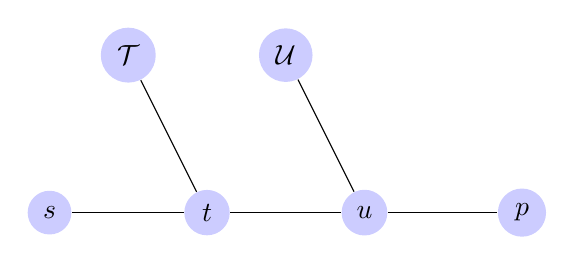
\begin{tikzpicture}
	[scale=1,every node/.style={circle,fill=blue!20}]
	\node (n1) at (1,1) {$s$};
	\node (n2) at (3,1) {$t$};
	\node (n3) at (5,1) {$u$};
	\node (n4) at (4,3) {$\mathcal{U}$};
	\node (n5) at (7,1) {$p$};
	\node (n6) at (2,3) {$\mathcal{T}$};
	\foreach \from/\to in {n1/n2,n2/n3,n3/n5,n4/n3,n6/n2}
	\draw (\from) -- (\to);
\end{tikzpicture}
\caption{Message passing in BP: first from $s$ to $t$ and from $\pi_t$ to $t$ }
\label{fig1}
\end{figure}

\item[Step 4:] Outward pass from the root to all the leaves. 
\end{description}

This algorithm allows us to compute min-marginals on a tree for, say node $u$ and label $j$:
\begin{equation}
\min_{\mathbf{x}} \{ E(\mathbf{x}) | x_u = j \} = \theta_u(j) + M^{p \rightarrow q}(j) + \sum_{q \in \mathcal{U}\cup \{t\}}M^{q\rightarrow u}(j)
\label{eq:}
\end{equation}
In a general graph, we use the same rules but it might not converge.



\subsection{TRW-S algorithm}

The energy minimization is NP-hard, so we relax the constraints: 
\begin{equation}
x_p\in\{0,1\} \Rightarrow x_p\in[0,1]
\label{eq:}
\end{equation}
and we try to solve the dual problem of this new linear program problem. For this we formulate lower bounds on the function and maximize the bound. Improvement of TRW-S is that \textbf{the bound never decreases}. Recall that our goal is to compute:
\begin{equation}
\Phi(\mathbf{x}) = \min_{\mathbf{x}} E(\mathbf{x}|\theta)
\label{eq:}
\end{equation}
The key idea is to:
%%%%%%%%%%%%%%%%%%%%%% FRAME 6 %%%%%%%%%%%%%%%%%%%%%%
\begin{enumerate}
	\item Split $\theta$ in $\theta_1 + \theta_2 + \cdots$;
	\item Compute minimum for each component: 
	\begin{equation}
	\Phi_i(\mathbf{x}) = \min_{\mathbf{x}} E(\mathbf{x}|\theta_i)
	\label{eq:}
	\end{equation}
	\item Combine the $\theta_i$ to get an actual bound on $\Phi$.
\end{enumerate}

\begin{figure}[h!]
\centering
\begin{tikzpicture}
	[scale=1,every node/.style={circle,fill=blue!20}]
	\node (n1) at (1,3) {};
	\node (n2) at (3,5) {};
	\node (n3) at (3,1) {};
	\node (n4) at (5,3) {};
	
	\node (n5) at (8,3) {};
	\node (n6) at (10,5) {};
	\node (n7) at (12,3) {};
	
	\node (n8) at (15,3) {};
	\node (n9) at (17,1) {};
	\node (n10) at (19,3) {};
	\foreach \from/\to in {n1/n2,n1/n3,n3/n4,n2/n4, n5/n6,n6/n7, n8/n9,n9/n10}
	\draw (\from) -- (\to);
\end{tikzpicture}
\caption{Decomposition of a graph $\mathcal{G}$ into trees $T$ and $T'$}
\label{fig1}
\end{figure}
We can re-write the parameter $\theta$ as a combination of $\theta^T$ defined on the trees $T$ and $T'$:
\begin{equation}
\begin{array}{rll}
	\theta & \equiv & \displaystyle \frac{1}{2} \theta^T + \frac{1}{2} \theta^{T'} \\
	\Phi(\theta) & \geq & \displaystyle \frac{1}{2} \Phi(\theta^T) + \frac{1}{2} \Phi(\theta^{T'}) 
\end{array}
\label{eq:}
\end{equation}
If we maximize the term on the right, we get a so-called 'lower bound' on the energy. The first idea is now to run a BP algorithm on each tree, but that does not impose that the energy never decreases. Hence the TRW-S makes up for this issue by \textbf{node averaging}. \\

Say for a node $s\in\mathcal{V}$ we have $s\in T \cap T'$ and say the value in $s$ is in $T$ (4,1) and in $T'$ (0,2), then when we recombine the initial graph, we associate to $s$ (2,1.5) (if $s$ is not in any other $\tilde{T}$). Here is the idea of TRW-S:
 
\begin{algorithm}
\caption{TRW-S algorithm}
\label{trws}
\begin{algorithmic}
\Require graph $\mathcal{G} = ( \mathcal{V}, \mathcal{E})$ with energy $E(\mathbf{x}|\theta)$
\Ensure $E^*$ lower bound on the energy

\State decompose $\mathcal{G}$ into trees $T\in\mathcal{T}$ entirely covering $\mathcal{G}$.
\For{$p \in \mathcal{V}$}
	\State Run BP on all trees $T$ such that $p\in T$
	\State Average node $p$
\EndFor
\end{algorithmic}
\end{algorithm}

\begin{center}
	\textbf{It is proved that the lower bound never decreases this way.}
\end{center}
As for implementation, running BP on all trees is inefficient because we can reuse on the order of nodes in BP to get a faster algorithm. It suffices to consider a smart order on the tree $T$ so that $p$ can be computed with just the inward pass, take the root. Then the algorithm is in $O(n)$ for each BP run. 















\newpage
%%%%%%%%%%%%%%%%%%%%%% FRAME 7 %%%%%%%%%%%%%%%%%%%%%%


\section{Implementation and Results}

The implementation has been done with python2.7. The svm part use the implementation of the library \textbf{scikit-learn}. We have used the implementation of TRW-S of the libraries\textbf{Opengm} and \textbf{TRW-S.1-3} you can find on the web.

To tune the SVM parameters, we have used a per-character grid-search over the parameters of regularization $C$ and the localization of our RBF kernel $\gamma$. This allows us to gain a character detection of $10\%$ while testing on our training set.

We use a simple process to test our implementation. We started with the simplest case of OCR, with a printed word on a white background, already localized. We then used harder images as our results got better.

\begin{figure}[ht!c]
\includegraphics[width=0.3\columnwidth]{figures/dada1.png}
\includegraphics[width=0.3\columnwidth]{figures/dada2.png}%
\includegraphics[width=0.3\columnwidth]{figures/dada3.png}%
\caption{Test on an artificial word 'dada'. Word retrieved: 'dda' or 'dd depending on the lexicon prior used}
\label{dada}
\vspace{0.5cm}
\centering
\includegraphics[width=0.4\columnwidth]{figures/puffTest.png}
\hspace{0.3cm}
\includegraphics[width=0.4\columnwidth]{figures/puff.png}%
\caption{Natural testing word. Word retrieved: 'PE'}%
\label{Puff}
\vspace{0.5cm}
\centering
\includegraphics[width=6cm]{figures/00_00.jpg}
\hspace{0.3cm}
\includegraphics[width=6cm]{figures/beerResized.png}%
\caption{Natural testing image}%
\label{beer}
\end{figure}

We can see in the Fig.(\ref{dada}) that most of the time there are way too many characters that are detected but we are 'practically' able to select the correct ones with the graphical model. In the Fig.(\ref{Puff}), we can see two problems. The first one is the F is detected as a E by our SVM because of shadows perhaps. Then, the graphical model penalizes the overlap too much and we end up with separated characters instead of a word detection. Indeed the energies introduce a term increasing as the overlapping gets bigger, to indeed avoid finding say a r instead of a n (very close is juste move left the sliding window) as the NMS is character specific. But it seems the tuning of those parameters is tricky as penalizing too much the overlapping leads to single separated characters instead of a whole word. The Fig.(\ref{beer}) shows that with bigger images and multiple scale, we got a graphical model too complicated and lost the intrinsic information.


\section{Improvements}

\begin{itemize}
\item The SVM performance is very low here even after a large cross-validation process. A first step would be to build a more robust character detection. One idea would be to pre-select the sliding windows based on the score of a character detector model. This could still be imprecise as there is a big variability over the characters.

\item Another observation we can make is that the model has no term in the energy that encourages words bigger than one letter in the energy. We can often observe that the resulting word are single separated characters whereas we are looking for a whole word.
\begin{figure}[hc!]
\centering
\includegraphics[width=0.3\columnwidth]{figures/beer2.png}
\caption{Spreading of the detected characters}
\end{figure}

\item The prior we use here is a bi-gram prior. It only take into account the succession of letter. One information we are not using is the fact that a 'P' is more frequent at the beginning of a word that at the end. We could thus follow the idea given in the paper \cite{Mis} to build a Node-specific prior. The idea is to compute for each graphical model a prior based on the place of the node in the image and in the graphical model. But this seem to be only possible after a cleaning of the graphical model in the first step. We should reduce the false positive rate and then extract all the connected components of our graph to build our lexical prior in this context.
\end{itemize}










%%%%%%%%%%%%%%%%%%%%%% FRAME 8 %%%%%%%%%%%%%%%%%%%%%%




\bibliographystyle{unsrt}
\bibliography{biblio}



\end{document}